\documentclass[10pt]{exam}
\usepackage[hon]{template-for-exam}
\usepackage{tikz,graphicx,multicol}

\title{Series vs. Parallel Lab}
\author{Rohrbach}
\date{\today}

\begin{document}
\maketitle

\begin{questions}
  \question
    \textbf{Pre-Lab:} Study the circuits below and describe whether they are series or parallel and how many bulbs will light up.

    \begin{tikzpicture}
      \node at (-4, 3) {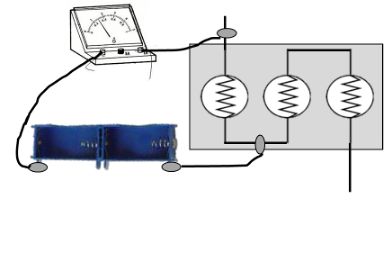
\includegraphics{circuit1.png}};
      \node at ( 4, 3) {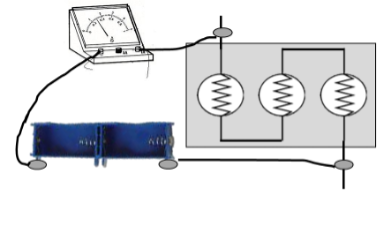
\includegraphics{circuit2.png}};
      \node at (-4,-3) {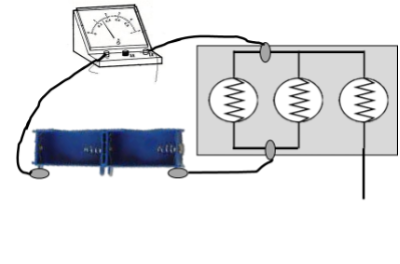
\includegraphics{circuit3.png}};
      \node at ( 4,-3) {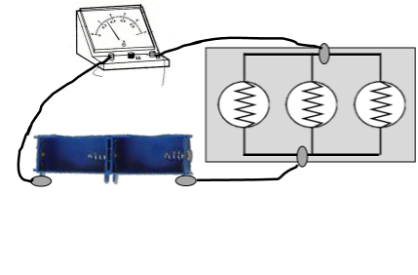
\includegraphics{circuit4.png}};
      \draw (-7,0) -- (7,0);
      \draw (0,-5) -- (0,5);
    \end{tikzpicture}

\uplevel{
  In this lab, you are going to light up one bulb, two bulbs, and three bulbs in \emph{series} and in \emph{parallel}.  You will use the multimeter to measure the \emph{current} running through the battery.
}

  \question
    Using the description above, what are your \emph{independent} and \emph{dependent} variables in this lab? \vs
  
  \question
    \textbf{Purpose:} Write one sentence explaining what you are trying to figure out in this lab.  Make sure your purpose includes all of your independent and dependent variables \vs

  \question
    \textbf{Hypotheses:} What do you predict will happen to the current through the battery as more light bulbs are added?  Do you think it will matter whether the bulbs are in series or parallel?  How so? \vs

  \pagebreak

  \question
    \textbf{Data:} Show all data tables for each of your experiments.  

    \renewcommand{\arraystretch}{2}

    \begin{multicols}{2}
      Current Through a Series Circuit

      \begin{tabular}{|c|c|}
        \hline
        \# of bulbs & current (amps) \\\hline
        1 &\\\hline
        2 &\\\hline
        3 &\\\hline
      \end{tabular}

      Current Through a Parallel Circuit

      \begin{tabular}{|c|c|}
        \hline
        \# of bulbs & current (amps) \\\hline
        1 &\\\hline
        2 &\\\hline
        3 &\\\hline
      \end{tabular}

    \end{multicols}

\question
  Create two scatter plots for your data


    \begin{multicols}{2}
      Current Through a Series Circuit

      \begin{tikzpicture}
        \draw[dotted] (0,0) grid[step=0.5] (7.5,6.5);
      \end{tikzpicture}

      Current Through a Parallel Circuit

      \begin{tikzpicture}
        \draw[dotted] (0,0) grid[step=0.5] (7.5,6.5);
      \end{tikzpicture}

    \end{multicols}
                 
\question
  \textbf{Results:} What was the relationship between your independent variable and your dependent variable (\emph{i.e.} directly proportional, inversely proportional, no effect, unclear) for each setup?  Did they match your hypothesis?
  \vs

\question
  \textbf{Conclusions:}  What happens when more bulbs are added in series?  In parallel?  Why does this make sense?
  \vs

  
\end{questions}


\end{document}